\documentclass[conference]{IEEEtran}
\IEEEoverridecommandlockouts
\usepackage{cite}
\usepackage{amsmath,amssymb,amsfonts}
\usepackage{booktabs}
\usepackage{enumitem}
\usepackage{tikz}
\usetikzlibrary{arrows.meta,positioning}

\newcommand{\sat}{\operatorname{sat}}
\newcommand{\diag}{\operatorname{diag}}

\begin{document}

\title{Quanser QArm Mini 4-DOF Manipulator:\\ Hardware Physics, Identification, Modelling, and the Complete Controller Suite\\
{\footnotesize Mathematical foundations for offline simulation, digital-twin, and hardware execution}}

\author{\IEEEauthorblockN{Gandhi Contreras}
\IEEEauthorblockA{\textit{Electrical and Computer Engineering}, New Mexico State University, Las Cruces, NM, USA \\ gandhico@nmsu.edu}}

\maketitle

\begin{abstract}
The QArm Mini is a desktop-scale four-revolute-joint manipulator actuated by integrated hobby-class smart servos whose embedded position loops are, for most operating modes, the only actuation interface exposed to the user. This changes the control mathematics in a specific, honest way: torque is not directly assignable, so the plant seen by the outer controller is the cascade of servo closed loops coupled by rigid-body dynamics acting as inter-joint disturbances. This paper develops the platform end to end under that reality: the scaling physics that make small arms drivetrain-dominated, the smart-servo and serial-bus physics, the serial-chain kinematics and Euler--Lagrange dynamics (identical in structure to the full-size arm), identification reformulated around the servo closed loops and gravity deflection, and the controller suite --- PID, LQR, LQG, backstepping, sliding mode, and NMPC --- each stated in its position-mode realization, where model-based torque laws become inverse-dynamics reference shaping. The safety envelope of a human-shared desktop arm completes the treatment.
\end{abstract}

\begin{IEEEkeywords}
QArm Mini, smart servos, position-mode control, scaling laws, serial manipulator, reference shaping, LQR, LQG, SMC, NMPC.
\end{IEEEkeywords}

%====================================================================
\section{Introduction}
The QArm Mini reproduces the anthropomorphic layout of its full-size sibling --- base yaw $q_1$, shoulder $q_2$, elbow $q_3$, wrist $q_4$, plus gripper --- at desktop scale. Its mathematical interest is not merely a smaller copy: the actuation interface (embedded position-mode servo loops over a serial bus) and the scaling laws below alter which physical effects dominate and how the classical controller suite is \emph{realized}. Throughout, $q\in\mathbb R^4$, end effector $x = f(q)$, Jacobian $J(q) = \partial f/\partial q$.

%====================================================================
\section{Hardware Physics}

\begin{figure*}[!t]
\centering
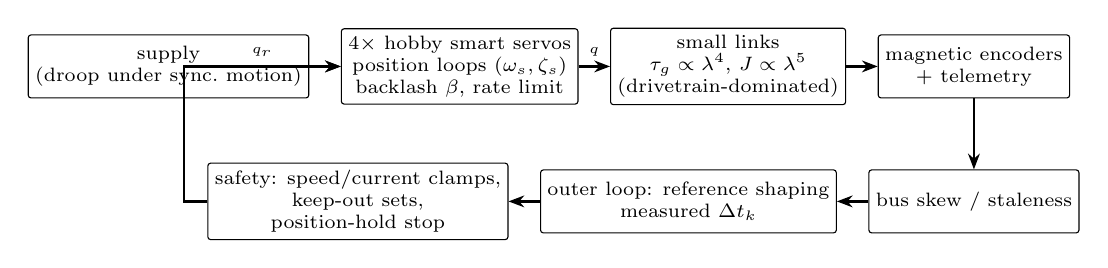
\begin{tikzpicture}[
  node distance=3mm and 4mm,
  blk/.style={draw, rounded corners=1pt, align=center, font=\scriptsize, inner sep=2.5pt, minimum height=8mm},
  lbl/.style={font=\tiny, align=center},
  arr/.style={-{Stealth[length=2mm]}, thick}
]

\node[blk] (sup) {supply\\ (droop under sync.\ motion)};
\node[blk, right=of sup] (srv) {$4\times$ hobby smart servos\\ position loops $(\omega_s,\zeta_s)$\\ backlash $\beta$, rate limit};
\node[blk, right=of srv] (links) {small links\\ $\tau_g\propto\lambda^4$, $J\propto\lambda^5$\\ (drivetrain-dominated)};
\node[blk, right=of links] (enc) {magnetic encoders\\ + telemetry};
\node[blk, below=9mm of enc] (bus) {bus skew / staleness};
\node[blk, left=of bus] (loop) {outer loop: reference shaping\\ measured $\Delta t_k$};
\node[blk, left=of loop] (safe) {safety: speed/current clamps,\\ keep-out sets,\\ position-hold stop};
\draw[arr] (sup) -- (srv);
\draw[arr] (srv) -- node[lbl, above] {$q$} (links);
\draw[arr] (links) -- (enc);
\draw[arr] (enc) -- (bus);
\draw[arr] (bus) -- (loop);
\draw[arr] (loop) -- (safe);
\draw[arr] (safe.west) -- ++(-3mm,0) |- node[lbl, pos=0.75, above] {$q_r$} (srv.west);
\end{tikzpicture}
\caption{QArm Mini signal chain: position-mode servo loops are the actuation interface; scaling laws make the decoupled realization near-exact; the outer controller shapes references.}
\label{fig:chain}
\end{figure*}
\subsection{Scaling laws: why small arms are drivetrain-dominated}
Under geometric scaling by factor $\lambda < 1$ (the Mini relative to a full-size arm): link masses scale as $m \propto \lambda^3$, gravity torques as $\tau_g \propto m g L \propto \lambda^4$, and link inertias as $J_{\mathrm{link}} \propto m L^2 \propto \lambda^5$. Meanwhile the reflected drivetrain inertia $N^2 J_m$ of the servo does not shrink with the links. Two consequences with control weight:
\begin{enumerate}[label=(\alph*)]
\item the inertia matrix is increasingly \emph{diagonal and configuration-independent} --- the reflected servo terms dominate the configuration-dependent link coupling, so per-joint (decentralized) control is closer to exact than on any larger arm;
\item gravity torques, while small in absolute terms, remain the largest \emph{sustained} load, and the servos' continuous-torque (thermal) rating --- not their peak torque --- is the binding actuation constraint for held postures.
\end{enumerate}

\subsection{Smart-servo modules and bus}
Each joint is an integrated module: coreless or cored DC micro-motor, gear train of ratio $N\!\sim\!10^2$ (spur/planetary; unlike the capstan drives of haptic devices, with measurable backlash $\beta$ at the output), magnetic absolute encoder, temperature and current telemetry, and an embedded controller closing a position (optionally velocity/current-limited) loop at kilohertz rate. The physics exposed to the outside:
\begin{equation}
\ddot q_j = \text{servo}_j(q_{r,j}) \;\Longrightarrow\;
q_j(s) \approx \frac{\omega_{s,j}^2}{s^2 + 2\zeta_{s,j}\omega_{s,j} s + \omega_{s,j}^2}\, q_{r,j}(s),
\label{eq:servo_tf}
\end{equation}
a well-damped second-order (or first-order-dominant) reference-to-angle response per joint, valid while the internal torque limit is inactive; when it saturates, the response degrades to rate limiting at $\dot q_{\max}(\tau_{\mathrm{load}})$, load-dependent through the speed--torque line of the DC motor, $\dot q_{\max} = \dot q_0(1 - \tau_{\mathrm{load}}/\tau_{\mathrm{stall}})$. Backlash $\beta$ appears as a dead zone in the load path --- position accuracy at the tool is bounded below by $\sum_j \beta_j\,\|\partial f/\partial q_j\|$ regardless of servo resolution. Manual-verified joint envelope (QArm Mini): asymmetric ranges base $-90^\circ/{+}225^\circ$, shoulder $0^\circ/{+}180^\circ$, elbow $0^\circ/{-}135^\circ$, wrist $0^\circ/{+}135^\circ$; maximum speed $\pi/2$~rad/s, acceleration $\pi/3$~rad/s$^2$; instantaneous/continuous torque $10.6/2.65$~N\,m at the shoulder and $4.1/1.0$~N\,m at base/elbow/wrist, gripper $1.9/0.5$~N\,m (instantaneous $\le0.1$~s); payload $150$~g for $15{+}$~min (unloaded indefinite), motor temperature limit $50^\circ$C --- the numbers behind the thermal budget of the NMPC formulation.

The half-duplex serial bus polls joints sequentially: the outer loop period $T_s$ is bus-bound (hundreds of hertz), commands and measurements of different joints are skewed within one cycle, and staleness enters as a per-joint delay $\tau_{d,j} < T_s$. All discrete updates in the outer controller advance on the \emph{measured} $\Delta t_k$, the discipline common to all of our platforms.

\subsection{Power path and safety}
A single DC supply feeds all modules through the bus harness; simultaneous multi-joint accelerations produce supply droop that momentarily lowers every servo's torque ceiling --- a matched disturbance visible in synchronized motions. Safety envelope for a desktop, human-shared arm: joint software limits inside the mechanical stops; Cartesian keep-out (table plane, self-collision cones); speed and current (hence force) clamps sized so that worst-case tool kinetic energy and pinch forces remain below injury thresholds --- the scaling laws make this achievable by configuration rather than by external safeguarding; thermal derating on sustained holds; bus-watchdog with \emph{position-hold} (never torque-free) stop, since the arm back-drives under gravity only marginally but the gripper payload may not be self-locking.

%====================================================================
\section{Kinematics and Dynamics}
\subsection{Kinematics}
Identical in structure to the full-size arm: base yaw selects the vertical working plane, $q_1 = \operatorname{atan2}(y, x)$; the planar shoulder--elbow pair solves in closed form,
\begin{equation}
\cos q_3 = \frac{r^2 + z^2 - l_2^2 - l_3^2}{2 l_2 l_3},\;\;
q_2 = \operatorname{atan2}(z, r) - \operatorname{atan2}(l_3 s_3, l_2 + l_3 c_3),
\end{equation}
elbow-up/down branches; the wrist disposes tool pitch. Singularities (stretched/folded $s_3 = 0$; wrist over the base axis $r = 0$) are handled by damped least squares in resolved-rate use, $\dot q = J^{\!\top}(JJ^{\!\top} + \lambda^2 I)^{-1}\dot x$.

\subsection{Dynamics}
The Euler--Lagrange form is structurally that of any serial arm,
\begin{equation}
M(q)\ddot q + C(q,\dot q)\dot q + G(q) + F_v\dot q + \tau_c\tanh(\dot q/\epsilon) = \tau,
\label{eq:minidyn}
\end{equation}
$M = M^{\!\top}\succ0$ with the reflected servo inertias on the diagonal, $\dot M - 2C$ skew-symmetric, $G(q)$ loading shoulder and elbow through elevation cosines. The scaling analysis makes the Mini-specific approximation quantitative:
\begin{equation}
M(q) \approx \bar M = \diag\bigl(N^2 J_{m,j} + \bar J_j\bigr),\qquad
\|M(q) - \bar M\| = O(\lambda^5),
\end{equation}
so \eqref{eq:minidyn} is, to leading order, four decoupled servo-inertia channels driven by gravity $O(\lambda^4)$ and friction --- the mathematical statement of ``drivetrain-dominated,'' and the licence for the decentralized designs below, with the coupling terms retained as the bounded disturbance they are.

\subsection{The plant seen by the outer controller}
In position mode the torque $\tau$ in \eqref{eq:minidyn} is generated internally by the servo loops. The outer plant is the map $q_r \mapsto q$: per joint the nominal response \eqref{eq:servo_tf}, perturbed by (i) gravity and coupling torques entering as load disturbances through the servo's finite stiffness, (ii) the torque/rate limits, and (iii) backlash. The \emph{static} manifestation of (i) is the gravity deflection
\begin{equation}
\delta q_j^{\mathrm{grav}}(q) = \frac{G_j(q) }{k_{P,j}^{\mathrm{servo}}},
\label{eq:sag}
\end{equation}
the sag of a proportional servo under load --- directly measurable, and the quantity that model-based reference shaping cancels.

%====================================================================
\section{Identification}

\begin{figure}[!t]
\centering
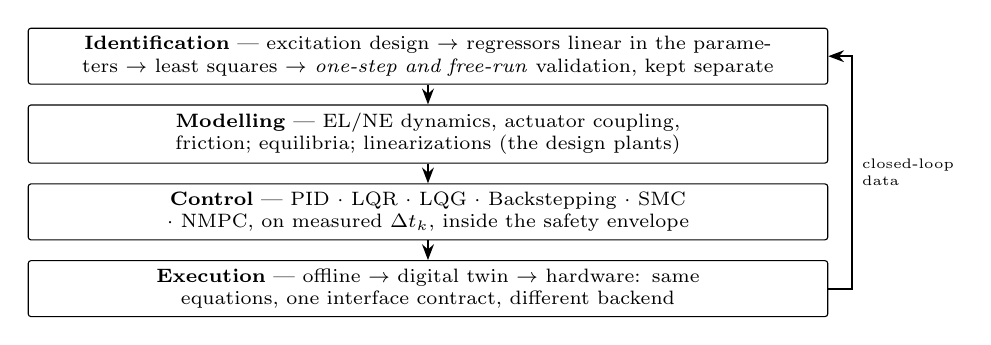
\begin{tikzpicture}[
  node distance=2.5mm,
  blk/.style={draw, rounded corners=1pt, align=center, font=\scriptsize, inner sep=3pt, text width=0.82\columnwidth},
  arr/.style={-{Stealth[length=2mm]}, thick}
]
\node[blk] (id) {\textbf{Identification} --- excitation design $\to$ regressors linear in the parameters $\to$ least squares $\to$ \emph{one-step and free-run} validation, kept separate};
\node[blk, below=of id] (mod) {\textbf{Modelling} --- EL/NE dynamics, actuator coupling, friction; equilibria; linearizations (the design plants)};
\node[blk, below=of mod] (ctl) {\textbf{Control} --- PID $\cdot$ LQR $\cdot$ LQG $\cdot$ Backstepping $\cdot$ SMC $\cdot$ NMPC, on measured $\Delta t_k$, inside the safety envelope};
\node[blk, below=of ctl] (exe) {\textbf{Execution} --- offline $\to$ digital twin $\to$ hardware: same equations, one interface contract, different backend};
\draw[arr] (id) -- (mod);
\draw[arr] (mod) -- (ctl);
\draw[arr] (ctl) -- (exe);
\draw[arr] (exe.east) -- ++(3mm,0) |- node[font=\tiny, pos=0.25, right, align=left] {closed-loop\\ data} (id.east);
\end{tikzpicture}
\caption{The workflow every platform in this series follows: identification feeds modelling, modelling feeds the controller suite, and all stages run unchanged across the three execution targets; closed-loop records return to identification.}
\label{fig:workflow}
\end{figure}
Reformulated for opaque embedded loops:
\begin{enumerate}[label=E\arabic*)]
\item \emph{Servo closed-loop response}: per joint, small reference steps and multisines about several postures; fit \eqref{eq:servo_tf} $(\omega_s, \zeta_s)$ and the rate limit $\dot q_{\max}$ vs.\ load --- the parameters every outer design consumes.
\item \emph{Gravity and stiffness}: quasi-static postures spanning elevation; regress commanded-vs-measured angle differences against the gravity regressor: \eqref{eq:sag} is linear in the mass moments over $k_P^{\mathrm{servo}}$, yielding the ratio needed for sag compensation (and, with servo current telemetry, $G(q)$ itself, linear in the link mass moments).
\item \emph{Backlash}: slow reversal sweeps at the output; $\beta_j$ from the hysteresis width.
\item \emph{Coupling residual}: synchronized two-joint motions; the deviation of each joint from its single-joint response identifies the off-diagonal disturbance magnitude, validating the $O(\lambda^5)$ decoupling claim on this unit.
\item \emph{Validation}: held-out trajectories; one-step and free-run (reference replay) fits reported separately, per joint and at the tool through $f(q)$.
\end{enumerate}

%====================================================================
\section{Control Suite in Position-Mode Realization}
The suite retains its mathematical identity; what changes is the \emph{actuation variable}: laws that output torque are realized as reference shaping through the identified servo model --- stated explicitly below. All outer updates on measured $\Delta t_k$; commands respect rate, travel, and thermal clamps.

\subsection{PID}
Native: the embedded loops \emph{are} PID; outer PID on task error (e.g., Cartesian correction mapped through $J^{-1}$) runs at the bus rate with anti-windup against the rate limit. Gravity-sag compensation is the first model injection:
\begin{equation}
q_r = q_d + \widehat{\delta q}^{\mathrm{grav}}(q_d),
\end{equation}
feedforward from E2 --- the position-mode analogue of gravity compensation.

\subsection{LQR / LQG}
Per joint, on the identified servo model \eqref{eq:servo_tf} augmented with the outer integrator: state $[\tilde q,\ \dot{\tilde q},\ \int\tilde q]$, input the reference increment $\Delta q_r$; the CARE gain shapes the closed outer loop subject to the inner loop's bandwidth ceiling $\omega_s$ (the outer crossover must sit a factor of 3--5 below $\omega_s$ --- the cascade rule made quantitative by the phase budget including $\tau_d$). LQG adds the Kalman filter over encoder quantization and bus skew; separation nominal.

\subsection{Backstepping / computed torque as reference shaping}
The torque-mode law $\tau = M(\ddot q_d + K_d\dot e + K_p e) + C\dot q + G$ is realized by commanding the reference that makes the servo produce it: to leading (drivetrain-dominated) order the servo tracks $q_r$ with dynamics \eqref{eq:servo_tf}, so inverse-shaping the desired trajectory through the identified model,
\begin{equation}
q_{r,j} = q_{d,j} + \frac{1}{\omega_{s,j}^2}\,\ddot q_{d,j} + \frac{2\zeta_{s,j}}{\omega_{s,j}}\,\dot q_{d,j} + \widehat{\delta q}_j^{\mathrm{grav}},
\label{eq:refshape}
\end{equation}
cancels the servo lag and the gravity sag --- model-based feedforward that is the exact position-mode image of computed torque; the backstepping construction ($z_1 = e$, $z_2 = \dot e + c_1 z_1$, $V = \tfrac12\sum z_i^{\!\top}z_i$) then closes the residual with $\Delta q_r = -(c_2 z_2 + z_1)/\omega_s^2$ and inherits $\dot V \le -\sum c_i\|z_i\|^2$ up to the identified coupling residual of E4.

\subsection{Sliding mode}
On the tracking error through the servo lag: $s = \dot e + \lambda e$ with the switching action realized as a bounded reference offset,
\begin{equation}
\Delta q_r = -\frac{\eta}{\omega_s^2}\,\sat(s/\phi),
\end{equation}
gain sized to the E4 coupling residual plus backlash-induced equivalent disturbance $\beta\,\omega_s^2$; the boundary layer is mandatory here --- inside the backlash dead zone the sign of the load path is undefined, and a discontinuous law would hunt across it (audible chatter and gear wear).

\subsection{NMPC}
Receding horizon at the trajectory level: decision variables are the reference sequence $\{q_{r,k}\}$; the prediction model is \eqref{eq:servo_tf} per joint (RK4 or exact discretization) with the rate/torque limits and \eqref{eq:sag}; cost on tool-space error through $f(q)$ plus reference smoothness; constraints: joint travel, rate limits, Cartesian keep-out sets, and the thermal continuous-torque budget as an integral constraint. This is where the Mini's suite regains full strength: the optimizer respects exactly the limits that degrade the shaped-reference laws, at bus-rate horizons that are computationally light because the models are second order and decoupled.

%====================================================================
\section{Execution Modes and Conclusion}
Offline: \eqref{eq:minidyn} wrapped by the identified servo loops \eqref{eq:servo_tf} with backlash, rate limits, bus skew, and quantization injectable --- the twin of the \emph{interface}, not just the rigid bodies. Digital twin: the vendor virtual arm under the same joint reference/measurement contract (position-mode parity is the natural first validation). Hardware: the physical arm under the desktop safety envelope. The Mini's lesson is methodological: when the actuation interface is a position-mode servo, the classical torque-level suite survives intact as mathematics but is \emph{realized} through the identified inner loops --- reference shaping \eqref{eq:refshape} in place of torque assignment, with the scaling laws guaranteeing that the decoupled realization is close to exact. That statement, made quantitative by E1--E5, is the platform's single source of truth across offline, twin, and hardware targets.

\bibliographystyle{IEEEtran}
\begin{thebibliography}{9}
\bibitem{siciliano2009} B.~Siciliano, L.~Sciavicco, L.~Villani, and G.~Oriolo, \emph{Robotics: Modelling, Planning and Control}. Springer, 2009.
\bibitem{spong2006} M.~W. Spong, S.~Hutchinson, and M.~Vidyasagar, \emph{Robot Modeling and Control}. Wiley, 2006.
\bibitem{slotine1991} J.-J.~E. Slotine and W.~Li, \emph{Applied Nonlinear Control}. Prentice Hall, 1991.
\bibitem{quanser_qarm_mini} Quanser Consulting Inc., \emph{QArm Mini User Manual}, Markham, ON, Canada.
\bibitem{nordin2002} M.~Nordin and P.-O. Gutman, ``Controlling mechanical systems with backlash --- a survey,'' \emph{Automatica}, vol.~38, no.~10, 2002.
\bibitem{khalil2002} H.~K. Khalil, \emph{Nonlinear Systems}, 3rd ed. Prentice Hall, 2002.
\bibitem{rawlings2017} J.~B. Rawlings, D.~Q. Mayne, and M.~Diehl, \emph{Model Predictive Control}, 2nd ed. Nob Hill, 2017.
\end{thebibliography}

\end{document}
